\section{Auswertung}
\subsection{Bestimmung der Apparatekonstanten}

Bevor die Trägheitsmomente der verschiedenen Körper bestimmt werden können müssen die
Apparatekonstanten bestimmt werden. Das ist zum einen die Winkelrichtgröße D und
das Trägheitsmoment der Drillachse $I_D$.

Die Winkelrichtgröße wird mithilfe der Gleichung (4) bestimmt. Die Kraft wird im Abstand
von $r = \SI{4.3}{\centi\meter} = \SI{4.3e-2}{\meter}$ gemessen.


\begin{table}[H]
  \centering
  \caption{Tabelle mit den Messdaten für die Winkelrichtgröße}
  \begin{tabular}{c c c c}
    \toprule
    $\phi$ in Grad & $\phi$ in rad & $F \, \, \text{in} \, N$ &
    $D \, \, \text{in} \, 10^{-2} N \si{\meter}$ \\
    \midrule
    50 &  $\frac{5\pi}{18}$ & 0.42 & 2.07 \\
    60 &  $\frac{\pi}{3}$ & 0.56 & 2.23 \\
    80 &  $\frac{4\pi}{9}$ & 0.8 & 2.46 \\
    90 &  $\frac{\pi}{2} $ & 0.82 & 2.24 \\
    100 & $\frac{5\pi}{9}$ & 0.96 & 2.37 \\
    120 & $\frac{2\pi}{3}$ & 1.16 & 2.38 \\
    140 & $\frac{7\pi}{9}$ & 1.34 & 2.36 \\
    160 & $\frac{8\pi}{9}$ & 1.54 & 2.37 \\
    180 & $\pi           $ & 1.78 & 2.44 \\
    200 & $\frac{10\pi}{9}$ &   2 & 2.46 \\
    \bottomrule
  \end{tabular}
\end{table}

Der Mittelwert und der zugehörige Fehler der Winkelrichtgrößen wird nun mit
folgenden Gleichungen bestimmt:\\\\


$\bar{D} = \frac{1}{N} \sum_{i=0}^{N} D_i$\\\\

$\Delta \bar{D} = \frac{1}{\sqrt{N}\sqrt{N-1}} \sqrt{\sum_{i}(D_i-\bar{D})^2}$\\\\


Damit ergibt sich für die Winkelrichtgröße:

\centerline{$\bar{D} = \num{2.388(39)e-2} Nm$}

Nun muss noch das TräTrägheitsmoment der Drillachse bestimmt werden. Dazu muss
die Gleichung (3) für diesen Fall noch angepasst werden, da sich das gesamte
Trägheitsmoment aus dem der Drillachse und der zwei Massen zusammensetzt:

$I = I_D + 2(I_{zh} + ma^2) = I_D + 2(m \left( \frac{d^2}{16} + \frac{h^2}{12} \right)
ma^2)$

Die geometrischen Abmessungen der beiden Massen sind:

\begin{itemize}
  \item Masse m = \SI{222.5e-3}{\kilo\gram}
  \item Höhe h = \SI{0.03}{\meter}
  \item Durchmesser d = \SI{0.035}{\meter}
\end{itemize}

Damit ergibt sich für das Trägheitsmoment der Massen:

\centerline{$I_{zh} = \SI{3.37e-5}{\kilo\gram\meter\squared}$}

Durch Umformung der Gleichung (3) folgt:

%$ \implies T^2 = 4 \pi^2 \frac{I}{D} = \frac{4\pi^2}{D}(I_D + 2(I_{zh} + ma^2))$\\
\begin{equation}
  T^2 = \frac{8\pi^2m}{D} a^2 + \frac{8\pi^2}{D} I_{zh} + \frac{4\pi^2}{D} I_D
\end{equation}


Das Trägheitsmoment der Drillachse wird nun mit einer Ausgleichsrechnung bestimmt.
Die Ausgleichsrechnung wird mit Python 3.6 durchgeführt.

\begin{table}
  \centering
  \caption{Tabelle mit den Messdaten für das Trägheitsmoment der Drillachse}
  \begin{tabular}{c c c c}
    \toprule
    $T$ in \si{\second} & $a$ in \SI{e-2}{\meter} & $T^2$ in \si{\second\squared} &
    $a^2$ in \SI{e-4}{\meter\squared} \\
    \midrule
    2.32 & 3.5  & 5.38  & 12.25 \\
    2.64 & 5.5  & 6.97  & 30.25 \\
    2.67 & 7.5  & 7.13  & 56.25 \\
    3.16 & 9.5  & 9.99  & 90.25 \\
    3.56 & 12.5 & 12.67 & 156.25 \\
    4.44 & 14.5 & 19.71 & 210.25 \\
    5.09 & 18.5 & 25.91 & 342.25 \\
    5.89 & 20.5 & 34.69 & 420.25 \\
    6.52 & 23.5 & 42.51 & 552.25 \\
    7.4  & 26.5 & 54.76 &  702.25 \\
    \bottomrule
  \end{tabular}
\end{table}

\begin{figure}[H]
  \centering
  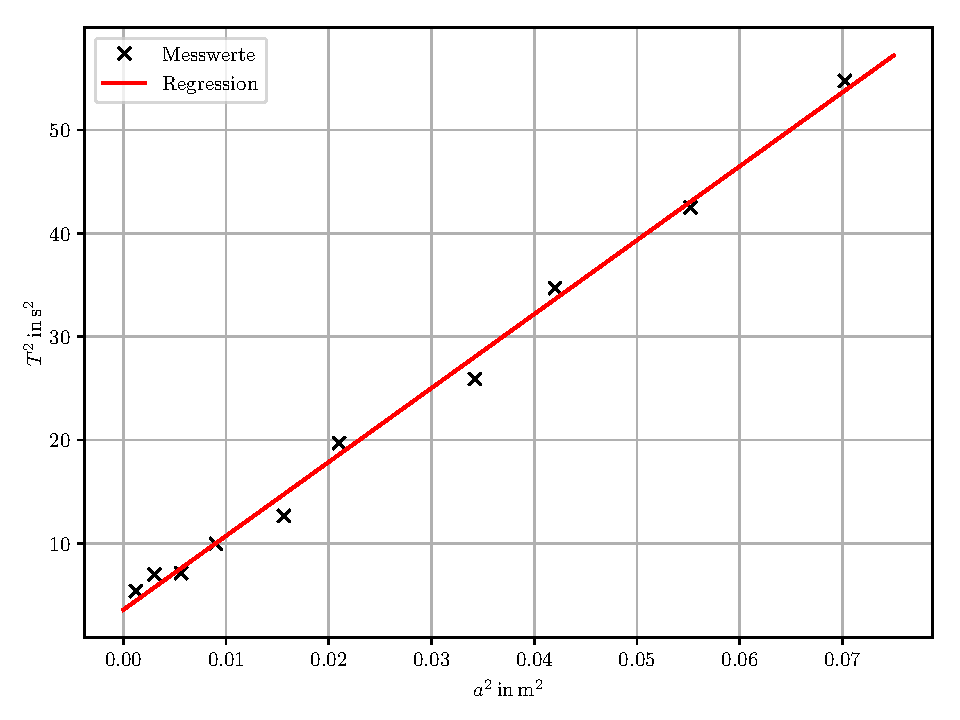
\includegraphics[width=\textwidth]{ausgleichsgerade1.pdf}
  \caption{Graphische Darstellung der Messwerte und der Ausgleichsgeraden}
\end{figure}

Damit ergeben sich die Parameter der Ausgleichsgeraden zu:

\begin{equation}
  y = m'x + b
\end{equation}

\begin{itemize}
  \item $m' = \SI{715.28(1921)}{\kilo\gram\per{\N\meter}}$
  \item $b = \SI{3.571(658)}{\kilo\gram\meter\per\N}$
\end{itemize}

Durch Vergleichen der Gleichungen (5) und (6) lässt sich das Trägheitsmoment der
Drillachse und die Winkelrichtgröße nochmal bestimmen.

\begin{gather}
  D_2 = \frac{8\pi^2m}{m'} \\
  I_D = \frac{D_2}{4\pi^2}b - 2I_{zh}
\end{gather}

Der Fehler der neu bestimmten Winkelrichtgröße wird mit der Gauß`schen Fehlerfortpflanzung
bestimmt:\\\\

$\Delta D_2 = \sqrt{\left(\frac{\partial D_2}{\partial m'} \cdot \Delta m' \right)^2}$\\\\
%= \frac{8\pi^2m}{m'^2} \cdot \Delta m'$

Die Winkelrichtgröße ist also:

\centerline{$D_2 = \SI{2.456(66)e-2}{\N\meter}$}

Damit kann nun das Trägheitsmoment der Drillachse bestimmt werden. Der Fehler wird
wieder mit der Gauß´schen Fehlerfortpflanzung bestimmt:\\\\

$\Delta I_D = \sqrt{\left(\frac{\partial I_D}{\partial D_2} \cdot \Delta D_2 \right)^2 +
\left(\frac{\partial I_D}{\partial b} \cdot \Delta b \right)^2}$\\\\

\centerline{$I_D = \SI{2.154(414)e-3}{\kilo\gram\meter\squared}$}

Mit den Apparatekonstanten kann nun das Trägheitsmoment von verschiedenen Körpern
mithilfe der Gleichung (3) bestimmt werden.


\subsection{Trägheitsmoment Kugel}

Um das Trägheitsmoment einer Kugel bestimmen zu können muss die Schwingungsdauer T
auf der Apparatur gemessen werden bei einer Auslenkung um einen bestimmten Winkel.
Dann ergibt sich das Trägheitsmoment zu:

\begin{equation}
  I_k = \frac{\bar{D}}{4\pi^2}\bar{T}^2 - I_D
\end{equation}

\begin{table}[H]
  \centering
  \caption{Tabelle mit den Messwerten für die Kugel}
  \begin{tabular}{c}
    \toprule
    T in \si{\second} \\
    \midrule
    1.61 \\
    1.41 \\
    1.67 \\
    1.63 \\
    1.49 \\
    \bottomrule
  \end{tabular}
\end{table}

Der Mittelwert der Schwingungsdauer mit der zugehörigen Standardabweichung
 wird mit den folgenden Gleichungen bestimmt:

$\bar{T} = \frac{1}{N} \sum_{i=0}^{N} T_i$\\\\

$\Delta \bar{T} = \frac{1}{\sqrt{N}\sqrt{N-1}} \sqrt{\sum_{i}(T_i-\bar{T})^2}$\\\\

 Somit ist der Mittelwert von den gemessenen T-Werten:

 \centerline{$\bar{T} = \SI{1.562(48)}{\second}$}

 Mit der Gleichung (9) lässt sich dann das Trägheitsmoment der Kugel bestimmen. Der
 zugehörige Fehler wird mit der Gauß´schen Fehlerfortpflanzung berechnet.\\\\

 $\Delta I_k = \sqrt{\left(\frac{\partial I_k}{\partial \bar{D}} \cdot \Delta \bar{D} \right)^2
  + \left(\frac{\partial I_k}{\partial \bar{T}} \cdot \Delta \bar{T} \right)^2
   + \left(\frac{\partial I_k}{\partial I_D} \cdot \Delta I_D \right)^2}$\\\\

\centerline{$I_k = \SI{-6.7817(42450)e-4}{\kilo\gram\meter\squared}$}

Das Trägheitsmoment der Kugel lässt sich auch mit dieser Gleichung berechnen:

\begin{equation}
I_k = \frac{2}{5} m \frac{D^2}{4}
\end{equation}

Die geometrischen Abmessungen der Kugel sind:

\begin{itemize}
  \item Masse: $m = \SI{812.5e-3}{\kilo\gram}$
  \item Durchmesser: $D = \SI{13.77e-2}{\meter}$
\end{itemize}

Damit ist das errechnete Trägheitsmoment der gleichen Kugel:

\centerline{$I_k = \SI{1.541e-3}{\kilo\gram\meter\squared}$}

\subsection{Trägheitsmoment Zylinder}

Die Gleichung zur Bestimmung des Trägheitsmoment von einen Zylinder lässt sich wieder
aus der Gleichung (3) herleiten.

\begin{equation}
  I_z = \frac{\bar{D}}{4\pi^2}\bar{T}^2 - I_D
\end{equation}

\begin{table}[H]
  \centering
  \caption{Tabelle mit den Messwerten für den Zylinder}
  \begin{tabular}{c}
    \toprule
    T in \si{\second} \\
    \midrule
    2.23 \\
    2.26 \\
    2.24 \\
    2.26 \\
    2.23 \\
    \bottomrule
  \end{tabular}
\end{table}

Die Messwerte der Schwingungsdauer müssen wieder gemittelt werden. Den Mittelwert
und die Standardabweichung werden mit den folgenden Gleichungen berechnet. \\\\

$\bar{T} = \frac{1}{N} \sum_{i=0}^{N} T_i$ \\\\

$\Delta \bar{T} = \frac{1}{\sqrt{N}\sqrt{N-1}} \sqrt{\sum_{i}(T_i-\bar{T})^2}$\\\\

Der Mittelwert der Schwingungsdauer ist also:

\centerline{$\bar{T} = \SI{2.244(7)}{\second}$}

Nun lässt sich das Trägheitsmoment des Zylinders bestimmen und den Feher mit Gauß´scher
Fehlerfortpflanzung:\\\\

$\Delta I_z = \sqrt{\left(\frac{\partial I_z}{\partial \bar{D}} \cdot \Delta \bar{D} \right)^2
 + \left(\frac{\partial I_z}{\partial \bar{T}} \cdot \Delta \bar{T} \right)^2
  + \left(\frac{\partial I_z}{\partial I_D} \cdot \Delta I_D \right)^2}$\\\\

Das Trägheitsmoment ist also:

\centerline{$I_z = \SI{8.9193(41741)e-4}{\kilo\gram\meter\squared}$}


Auch das Trägheitsmoment des Zylinders lässt sich auch wieder mithilfe der geometrischen
Abmessungen bestimmen:

\begin{equation}
  I_z = \frac{mD^2}{8}
\end{equation}

\begin{itemize}
  \item Masse: $m = \SI{2.3961}{\kilo\gram}$
  \item Durchmesser: $D = \SI{10.025e-2}{\meter}$
  \item Höhe: $h = \SI{14e-2}{\meter}$
\end{itemize}

Damit ergibt sich das Trägheitsmoment zu:

\centerline{$I_z = \SI{3.01e-3}{\kilo\gram\meter\squared}$}

\subsection{Trägheitsmoment der Puppe mit Arme zur Seite}

Das Trägheitsmoment der Puppe wird wieder genauso bestimmt wie bei den zwei anderen
geometrischen Figuren. Die Formel ist also:

\begin{equation}
  I_{p1} = \frac{\bar{D}}{4\pi^2}\bar{T}^2 - I_D
\end{equation}

\begin{table}[H]
  \centering
  \caption{Tabelle mit den Messwerten für die Puppe mit Armen zur Seite}
  \begin{tabular}{c}
    \toprule
    T in \si{\second} \\
    \midrule
    1.44 \\
    1.25 \\
    1.35 \\
    1.36 \\
    1.41 \\
    \bottomrule
  \end{tabular}
\end{table}

Der Mittelwert und die Standardabweichung der Schwingungsdauer müssen nun wieder
bestimmt werden.\\\\

$\bar{T} = \frac{1}{N} \sum_{i=0}^{N} T_i$ \\\\

$\Delta \bar{T} = \frac{1}{\sqrt{N}\sqrt{N-1}} \sqrt{\sum_{i}(T_i-\bar{T})^2}$\\\\

Der Mittelwert ist damit:

\centerline{$\bar{T} = \SI{1.362(32)}{\second}$}

Um den Fehler des Trägheitsmoments zu bestimmen muss wieder eine Gauß´sche
Fehlerfortpflanzung durchgeführt werden.\\\\

$\Delta I_{p1} = \sqrt{\left(\frac{\partial I_{p1}}{\partial \bar{D}} \cdot \Delta \bar{D} \right)^2
 + \left(\frac{\partial I_{p1}}{\partial \bar{T}} \cdot \Delta \bar{T} \right)^2
  + \left(\frac{\partial I_{p1}}{\partial I_D} \cdot \Delta I_D \right)^2}$\\\\

\centerline{$I_{p1} = \SI{-1.0319(4177)e-3}{\kilo\gram\meter\squared}$}

\subsection{Trägheitsmoment der Puppe mit Armen nach oben}

Zuletzt wird das Trägheitsmoment der Puppe in einer anderen Position bestimmt. In dem
fall hat die Puppe die Arme nach oben gestreckt. Die Formel zur berechnung des
Trägheitsmoments lässt sich wieder aus der Gleichung (3) herleiten.

\begin{equation}
  I_{p2} = \frac{\bar{D}}{4\pi^2}\bar{T}^2 - I_D
\end{equation}

\begin{table}[H]
  \centering
  \caption{Tabelle mit den Messwerten für die Puppe mit Armen nach oben}
  \begin{tabular}{c}
    \toprule
    T in \si{\second} \\
    \midrule
    0.76 \\
    0.46 \\
    0.46 \\
    0.44 \\
    0.45 \\
    \bottomrule
  \end{tabular}
\end{table}

Zur Berechnung des Trägheitsmomentes wird zunächst der Mittelwert und der Fehler
der Messungen bestimmt.\\\\

$\bar{T} = \frac{1}{N} \sum_{i=0}^{N} T_i$ \\\\

$\Delta \bar{T} = \frac{1}{\sqrt{N}\sqrt{N-1}} \sqrt{\sum_{i}(T_i-\bar{T})^2}$\\\\

Mithilfe dieser Formeln ergibt sich nun der Mittelwert:\\\\

\centerline{$\bar{T} = \SI{0.514(62)}{\second}$}

Für den Fehler des Trägheitsmomentes wird wieder die Gauß´sche Fehlerfortpflanzung
benutzt:\\\\

$\Delta I_{p2} = \sqrt{\left(\frac{\partial I_{p2}}{\partial \bar{D}} \cdot \Delta \bar{D} \right)^2
 + \left(\frac{\partial I_{p2}}{\partial \bar{T}} \cdot \Delta \bar{T} \right)^2
  + \left(\frac{\partial I_{p2}}{\partial I_D} \cdot \Delta I_D \right)^2}$\\\\

\centerline{$I_{p2} = \SI{-1.9942(4158)e-3}{\kilo\gram\meter\squared}$}

\subsection{Trägheitsmoment der Puppe über geometrische Abmessungen}

Auch bei der Puppe lässt sich wieder das Trägheitsmoment über die geometrischen
Abmessungen bestimmen, indem die einzelnen Körperteile als Zylinder angenommen werden.

\begin{table}[H]
  \centering
  \caption{Tabelle mit den Durchmessern für die Puppe}
  \begin{tabular}{c c c c}
    \toprule
    Kopf in \SI{e-2}{\meter} & Rumpf in \SI{e-2}{\meter} & Arm in \SI{e-2}{\meter} & Bein in \SI{e-2}{\meter} \\
    \midrule
     3.635 & 5.91 & 2.1  & 2.54\\
    3.44  & 5.62 & 2.09 & 2.18\\
    2.77  & 4.21 & 1.8  & 1.8 \\
    2.245 & 3.5  & 1.53 & 1.49\\
          & 4.7  & 1.92 & 2.35\\
          & 4.96 & 1.71 & 1.79 \\
          &      & 1.4  & 1.64 \\
    \bottomrule
  \end{tabular}
\end{table}

Die gemessenen Durchmesser müssen gemittelt werden und die Standardabweichung muss
bestimmt werden mit folgenden Formeln:\\\\

$\bar{d} = \frac{1}{N} \sum_{i=0}^{N} d_i$ \\\\

$\Delta \bar{d} = \frac{1}{\sqrt{N}\sqrt{N-1}} \sqrt{\sum_{i}(d_i-\bar{d})^2}$\\\\

Damit ergeben sich die geometrischen Abmessungen der Puppe zu:

\begin{itemize}
  \item Kopf:
    \begin{itemize}
      \item Höhe: $h = \SI{7e-2}{\meter}$
      \item Durchmesser: $\bar{d} = \SI{3.0225(3186)e-2}{\meter}$
    \end{itemize}
  \item Rumpf:
    \begin{itemize}
      \item Höhe: $h = \SI{12.03e-2}{\meter}$
      \item Durchmesser: $\bar{d} = \SI{4.817(364)e-2}{\meter}$
    \end{itemize}
  \item Arm:
    \begin{itemize}
      \item Höhe: $h = \SI{17.13e-2}{\meter}$
      \item Durchmesser: $\bar{d} = \SI{1.793(101)e-2}{\meter}$
    \end{itemize}
  \item Bein:
    \begin{itemize}
      \item Höhe: $h = \SI{18.99e-2}{\meter}$
      \item Durchmesser: $\bar{d} = \SI{1.97(15)e-2}{\meter}$
    \end{itemize}
\end{itemize}

Nun werden die Massen der einzelnen Körperteile bestimmt, aus der Gesamtmasse der
Puppe $m_{ges} = \SI{341.2e-3}{\kilo\gram}$. Dazu wird folgende Gleichung benutzt:

\begin{equation}
  \frac{V}{V_{ges}} = \frac{m}{m_{ges}} \iff m = \frac{V \cdot m_{ges}}{V_{ges}}
\end{equation}

Also müssen zunächst die Volumina der Körperteile berechnet werden. Da sie alle als
Zylinder angenommen werden kann die Formel $V = \frac{\pi}{4} \bar{d}^2 h$ dafür verwendet
werden.

Da die Durchmesser fehlerbehaftet sind muss der Fehler des Volumens mithilfe der
Gauß´schen Fehlerfortpflanzung berechnet werden.\\\\

$\Delta V = \sqrt{\left(\frac{\partial V}{\partial \bar{d}} \cdot \Delta \bar{d} \right)^2}$\\\\

\begin{itemize}
  \item Kopf: $V_k = \SI{5.0(11)e-5}{\meter\tothe{3}}$
  \item Rumpf: $V_r = \SI{21.9(33)e-5}{\meter\tothe{3}}$
  \item Arm: $V_a = \SI{4.3(5)e-5}{\meter\tothe{3}}$
  \item Bein: $V_b = \SI{5.8(9)e-5}{\meter\tothe{3}}$
\end{itemize}

Das Gesamtvolumen der Puppe ist damit:

\centerline{$V_{ges} = \SI{47(4)e-5}{\meter\tothe{3}}$}

Um mit der Gleichung (15) nun die eizelnen Massen zu bestimmen muss außerdem wieder
der Fehler der Massen mit der Gauß´schen Fehlerfortpflanzung berechnet werden:\\\\

$\Delta m = \sqrt{\left(\frac{\partial m}{\partial V} \cdot \Delta V \right)^2
  + \left(\frac{\partial m}{\partial V_{ges}} \cdot \Delta V_{ges} \right)^2}$\\\\

Die Massen der einzelnen Körperteile der Puppe sind:

\begin{itemize}
  \item Kopf: $m_k = \SI{4.1(13)e-3}{\kilo\gram}$
  \item Rumpf: $m_r = \SI{159(28)e-3}{\kilo\gram}$
  \item Arm: $m_a = \SI{31(4)e-3}{\kilo\gram}$
  \item Bein: $m_b = \SI{42(7)e-3}{\kilo\gram}$
\end{itemize}

Nun können die Trägheitsmomente der einzelnen Körperteile einzeln ausgerechnet werden
und zu dem Gesamtträgheitsmoment aufsummiert werden. Da die Puppe zwei unterschiedliche
Stellungen hat, wird diese Rechnung für beide Fälle einzeln durchgeführt.

\subsubsection{Puppe mit Armen zur Seite}

In diesem Fall geht die Drehachse nur durch den Schwerpunkt des Kopfes und des Rumpfes.
Die Trägheitsmomente von diesen beiden Körperteilen kann also mit der Gleichung (12)
bestimmt werden.

Der Fehler für diese beiden Trägheitsmomente wird mit folgender Formel berechnet:\\\\

$\Delta I = \sqrt{\left(\frac{\partial I}{\partial m} \cdot \Delta m \right)^2
  + \left(\frac{\partial I}{\partial \bar{d}} \cdot \Delta \bar{d} \right)^2}$\\\\

Für die Trägheitsmomente der Arme und der Beine muss der Steinersche Satz angewendet
werden. Der Schwerpunkt der Beine ist um $a = \frac{d_b}{2}$ von der Drehachse verschoben.
Damit ergibt sich für die Beine die Formel:\\\\

$I_b = \frac{m_b \bar{d_b}^2}{8} + m_b \frac{\bar{d_b}^2}{4}$\\\\

Der Fehler des Trägheitsmomentes der Beine wird mit der Gauß´schen Fehlerfortpflanzung
bestimmt: \\\\

$\Delta I_b = \sqrt{\left(\frac{\partial I_b}{\partial m_b} \cdot \Delta m_b \right)^2
  + \left(\frac{\partial I_b}{\partial \bar{d_b}} \cdot \Delta \bar{d_b} \right)^2}$\\\\

Der Schwerpunkt der Arme ist um $a = \frac{d_r}{2} + \frac{h_a}{2}$ von der Drehachse verschoben
und die Arme stehen auch anders zur Drehachse, deshalb lautet die Gleichung zur
bestimmung des Trägheitsmomentes der Arme: \\\\

$I = m \left( \frac{\bar{d}^2}{16} + \frac{h^2}{12} \right)$\\\\

Mit dem Steinerschen Satz folgt dann:\\\\

$I_a = m_a \left( \frac{\bar{d_a}^2}{16} + \frac{h_a^2}{12} \right)
+ m_a \left(\frac{\bar{d_r}}{2} + \frac{h_a}{2}\right)^2$ \\\\

Der Fehler des Trägheitsmomentes der Arme ergibt sich aus der Gauß´schen
Fehlerfortpflanzung: \\\\

$\Delta I_a = \sqrt{\left(\frac{\partial I_a}{\partial m_a} \cdot \Delta m_a \right)^2
  + \left(\frac{\partial I_a}{\partial \bar{d_a}} \cdot \Delta \bar{d_a} \right)^2
  + \left(\frac{\partial I_a}{\partial \bar{d_r}} \cdot \Delta \bar{d_r} \right)^2}$\\\\

Nun werden die einzelnen Trägheitsmomente der Körperteile bestimmt.

\begin{itemize}
  \item $I_k = \SI{4.1(13)e-6}{\kilo\gram\meter\squared}$
  \item $I_r = \SI{4.6(11)e-5}{\kilo\gram\meter\squared}$
  \item $I_a = \SI{2.82(5)e-3}{\kilo\gram\meter\squared}$
  \item $I_b = \SI{6.1(14)e-6}{\kilo\gram\meter\squared}$
\end{itemize}

Das gesamte Trägheitsmoment der Puppe in diesem Fall ist also:\\\\

\centerline{$I_{ges} = \SI{5.7(1)e-3}{\kilo\gram\meter\squared}$}

\subsubsection{Puppe mit Armen nach oben}

Da die Stellung von dem Kopf, dem Rumpf und den Beinen identisch zu den vorherigen
Fall ist, sind die Trägheitsmomente der genannten Körperteile auch gleich.
Nur das Trägheitsmoment der Arme muss neu bestimmt werden.

Nun ist der Schwerpunkt der Arme um den Abstand $a = \frac{d_r}{2} + \frac{d_a}{2}$
von der Drehachse verschoben. Außerdem ist die Stellung der Arme in diesem Fall anders,
deshalb kann die Gleichung (12) für den Steinerschen Satz verwendet werden.\\\\

$I_a = \frac{m_a \bar{d_a}^2}{8} + m_a \left( \frac{\bar{d_r}}{2} + \frac{\bar{d_a}}{2} \right)^2$\\\\

Der Fehler wird mit folgender Gleichung berechnet:\\\\

$\Delta I_a = \sqrt{\left(\frac{\partial I_a}{\partial m_a} \cdot \Delta m_a \right)^2
  + \left(\frac{\partial I_a}{\partial \bar{d_a}} \cdot \Delta \bar{d_a} \right)^2
  + \left(\frac{\partial I_a}{\partial \bar{d_r}} \cdot \Delta \bar{d_r} \right)^2}$\\\\

Damit ergibt sich für das neu bestimmte Trägheitsmoment der Arme:

\begin{itemize}
  \item $I_a = \SI{3.5(6)e-5}{\kilo\gram\meter\squared}$
\end{itemize}

Das gesamte Trägheitsmoment für diesen Fall ist damit:\\\\

\centerline{$I_{ges} = \SI{1.33(19)e-4}{\kilo\gram\meter\squared}$}
